\documentclass{llncs}


%\usepackage{todonotes}
\usepackage{url}
\usepackage{hyperref}
\usepackage{booktabs}
\usepackage{subfigure}

\usepackage{graphicx,url}
\usepackage{color}
\usepackage{xcolor}
\usepackage{epstopdf}
\usepackage{hyperref}
\usepackage{xspace}
\usepackage{times}

\newcommand{\jacamo}{\textsf{\small JaCaMo}\xspace}
\newcommand{\moise}{$\mathcal{M}$\textsf{\small oise}\xspace}
\newcommand{\cartago}{\textsf{\small CArtAgO}\xspace}

\begin{document}
\title{A Team for MAPC Considering the Organization and the Environment as First-class Abstractions\thanks{We are grateful for the support given by CAPES and CNPq (grant numbers 140261/2013-3, 306301/2012-1).}}
\author{Maicon R. Zatelli \and 
		Maiquel de Brito \and 
		Tiago L. Schmitz \and \\
		Marcelo M. Morato \and
		Kaio S. de Souza \and 
		Daniela M. Uez \and 
		Jomi F. H\"{u}bner }

\institute{Department of Automation and Systems Engineering \\ Federal University of Santa Catarina \\ CP 476, 88040-900 Florian\'{o}polis - SC - Brasil \\ 
\email{	{\scriptsize \{xsplyter,tiagolschmitz,marcelomenezes73,dani.uez\}@gmail.com, maiquel.b@posgrad.ufsc.br,kaiossouza@hotmail.com,jomi.hubner@ufsc.br}} }

\maketitle
\begin{abstract} 
This paper describes the SMADAS team for the Multi-Agent Programming Contest 2013. Throughout this paper we highlight the design, main strategies, tools, and results of our team. For this year we used the \jacamo\ platform to develop the team, which is composed of Jason (to program the agents), \cartago\ (to program the environment), and \moise\ (to program the organization). We also improved the last year team with new strategies focused on the updated ``Agents on Mars'' scenario.
\end{abstract}

% -------------------------------
% Inclusao dos capitulos do texto
% +- 1 pagina
\section{Introduction}

The Multi-Agent Programming Contest (MAPC)~\cite{koster:2013}\footnote{\url{http://multiagentcontest.org}} is an important event to stimulate research in the multi-agent systems programming field. The MAPC 2013 used the ``Agents on Mars'' scenario, which was improved from the last year scenario, therefore the efforts must continue concentrated in cooperation, coordination, and decentralization. Our agent team, called SMADAS, acronym for our research group, named Multi-Agent Systems from Systems and Automation Department (in Portuguese, \textbf{S}istemas \textbf{M}ulti\textbf{a}gentes  do \textbf{D}epartamento de \textbf{A}utoma\c{c}\~ao e \textbf{S}istemas) was developed by a group formed by one PhD, four PhD students, and two undergraduate students from the Federal University of Santa Catarina (UFSC). This is our second participation in the contest and we have two main aims this year: improve our MAS developing skills and evaluate some proposals developed in our thesis. 

 		
%+- 2 páginas
% Linguagem usada - pq? 
% Uso de metodologia:
%	Não foi usada nenhuma conhecida por causa da falta de experiência no uso de metodologias, porém foi usada uma de divisão do trabalho	
% Como foi dividido o trabalho no time?
% 	Reuniões quinzenais para definição de estratégias
%	Testes dos times com diferentes estratégias
%	Comparação com estratégias usadas anos anteriores.
%	Um responsável pelo desenvolvimento.
% 	Divisão do problema: primeiro exploração, depois exploitação, etc, etc...
% Tempo de desenvolvimento

\section{System Analysis and Design}
%an ad-hoc
For the analysis of our systems, we adopted a prototype driven approach instead of a well known software engineering methodology because the problem seemed quite simple to solve and we had no experience with them. Thus we decided that it was better to use our time developing the system than learning a methodology.

Based on the agent contest scenario description, we divided the overall problem in sub-problems, each one analysed in detail: exploration, exploitation, attack and defense, buy, repair, and inspection. A team member was engaged with programming each strategy discussed on biweekly meetings. Forty five versions of the system were produced in this phase. These versions were tested and compared with the best teams from the last contest \cite{dominic:2012,ettienne:2012,dekker:2012,behrens:2012} and also against our own versions of the system in order to select the most efficient one. In these preliminary tests, we identified some good strategies for the final implementation. To develop the SMADAS system, we spent about 500 hours, most of them testing the strategies.

The system has 20 agents of five types: repairer, saboteur, explorer, sentinel, and inspector. We considered two main distinct phases: exploration, in which the explorers identify all vertices and nodes in the map and find the best zones, and exploitation, where all agents try to conquest and defend these zones. During the match, if an agent senses a nearby enemy it calls a saboteur to attack it, and also if the agent is damaged it tries to find a repairer to be fixed. 

Our agents are able to decide their own actions, however this autonomy produces some conflicting situations like two agents deciding to exploit different zones. These situations are solved using a centralized approach, which consists of a specific agent been responsible for the group decision. For example, one of the explorers defines the zones to exploit and one of the repairers defines the reparation order. Some conflicting situations are simply prevented by using a predefined priority order among the agents, where agents with higher priorities acts before agents with less priority.

The coordination among the agents is based on two communication mechanisms: blackboard and message exchanging. The blackboard is used to provide a global graph view to the agents, since some important information about the graph structure is synchronized in it. We decided to use a blackboard because the agents need an overall view of the scenario to be able to define the system exploitation strategy. The message exchanging is used to share information about the inspected enemies, the ally agent actions and damages, and about the map zones. The communication protocol used when a damaged agent needs to be repaired is shown in Fig.~\ref{fig:protocol}. It consists of the agent asking a repairer that contacts the other repairers to find out which one is the closest to the damaged agent. Then the other repairers inform their positions and the closest one is selected to repair the damaged agent. Thus, the selected repairer will send to the damaged agent the meeting path. 


\begin{figure}
\centering 
 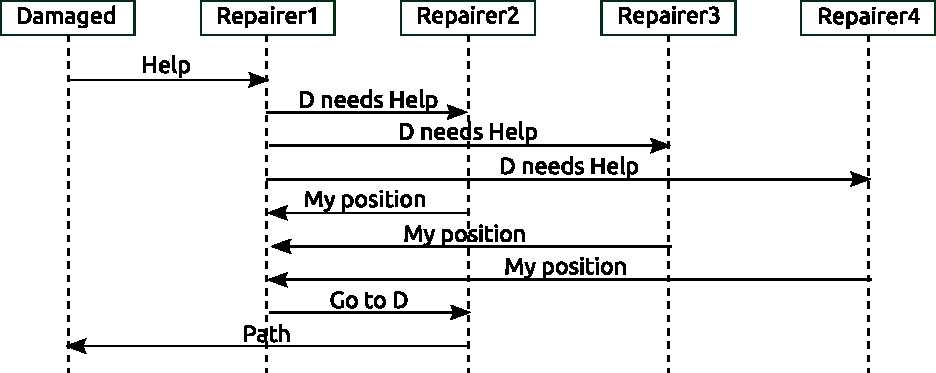
\includegraphics [width=0.9\linewidth] {./protocolo.pdf}
\caption{A communication protocol used to define which repairer will repair a damaged agent. The damaged agent asks the \texttt{repairer1} for help, the \texttt{repairer1} then contacts the others repairers to find which one is the closest to the damaged agent. All repairer send their position and the \texttt{repairer1} elects the closest one. The selected repairer then sends the meet point to the damaged agent.}
\label{fig:protocol}	
\end{figure}

The SMADAS system is a truly MAS because the agents are autonomous, reactive, and proactive. They have autonomy to decide how and when to execute most of their actions, except the few conflicting situations explained before. However, the agents also perform some actions in reaction to environment events, like the start of the step or a received message. Other reactive actions occurs when a saboteur attacks an enemy agent that is in the same vertex or when an agent runs away or defends itself from an enemy saboteur on the same vertex. Furthermore, the agents have a proactive behaviour, that shows up when they try to find a better vertex that improves the team score, contact the repairer when they are damaged, or look for enemies to attack. 


\section{Software Architecture}

As we done in the edition of 2012~\cite{smadas:2012}, in the current edition of MAPC we used the EISMASSim~\cite{behrens:2011} to communicate with the contest server. However, while in the previous edition the team was developed essentially using Jason, in the current edition, our team has been developed with \jacamo\  platform. This was the main change in the software architecture for this year. Furthermore, even with the increase number of agents, from 20 to 28, we were still able to run the agents in a single machine, therefore we decided to avoid distributing the agents between several machines. We also made several contributions for the tools that we used in this year. In Jason, we added features to handle goals with deadlines, new mechanisms for the \texttt{.wait} internal action, and we fixed some bugs. In \moise, we added a new feature to reset organizational goals to avoid creating new schemes at runtime and we added an organizational monitor accessed via HTTP, so that we were able to watch our team organization remotely.

The source code of the team has 3794 lines of Jason code, 135 for \moise, 96 for \cartago, and 4434 for Java, totaling 8459 lines. Although the implemented strategies of these year are more complex, we can notice that the number of lines coded in Jason has decreased from 5504 in last year's team to 3794 this year. It is an expected consequence of the organization and the environment programming available in \jacamo. Coordination strategies that previously required several lines of Jason code, could now be coded in a few lines of \moise, since \moise\ is a proper language for that.  Not only have we reduced the size of the programs, but the new approach has allowed us to debug and change the organization of the team quite easily. Instead of monitoring the agents internal state, we can now monitor the state of the organization, which is a more general view of the state of the team. Since the organizational program is the same as the specification, to change the team sometimes is simply reduced to update the organization. For instance, to change the order of organizational goals, we simply need to change the scheme of Fig.~\ref{fig:org_fs}.
% +- 3 paginas
% Como funciona cada agente?
% Prioridades de escolha
% - Estrategias de exploracao
% 	- Compartilhamento de informacoes
% - Exploitacao:
% 	- selecao de zonas, 2 morrinhos (por que usou 2 morrinhos?)
% - Compra: hulk - por que usamos? 
% - reparacao
% - ataque/defesa
% detalhes importantes da estrategia de jogo - se tiver
\section{Strategies}

% \item Is most of you agents' behavior emergent on and individual and team level?
% \item Do your agents have an explicit mental state? 
In our strategy both individual and group behavior are important. While the individual behavior is important when the agents are isolated in the map, the group behaviour is responsible for preventing redundant actions and for producing a coherent and cooperative global result. The agents are proactive in order to get achievement points and obtaining a good score. They also use their beliefs and the exchanged information to decide their next action.

%\item What is the main strategy of your team?
As commented in the previous section, we consider two main strategies: exploration and exploitation. In the exploration phase the agents just explore the map and try to get as most achievement points as possible. After step 15, our agents go to a good zone to conquer it.

% \item How important are achievements for your overall strategy?
Since achievement points are important and they accumulate in each one of the 750 steps, it is desirable to obtain them as soon as possible. However, some achievements are more complicated to conquer after some time, hence they can be ignored. For example, it does not make sense to survey all edges in the graph, considering it takes a long time to be performed. Instead of it, our agents stay in a vertex getting more score by exploiting water wells. For the same reason we are not interested on inspecting all opponent agents, thus our inspectors only inspect them when they are near.

%\item How do you find good zones? How do you estimate the value of zones?
After the exploration phase, the exploitation phase starts. One of our explorers reasons about which are the two best zones in the map to be exploited. Exploiting two zones is advantageous since the map is symmetric and it is particularly important against teams that keep only one zone. In order to do that, we used a modified version of the BFS algorithm, that is run for all vertex, summing their values until some depth. The vertex with the highest sum represents where the best zone is (zone 1). After it, the algorithm tries to find the second best vertex to set the second best zone (zone 2), which may have some intersection with the first one. This algorithm is not optimal because its result is always a circular shape, when the ideal choice often has a free shape.

%\item How do you conquer zones? How do you defend zones if attacked? Do you attack zones?

When the good zones are defined, an explorer organises the agents in two groups, one for zone 1 and another for zone 2. Each group has 10 members, with two agents of each type. The agents are then informed about the central vertex of its zone and how far they can go from it. The central vertex of an area is the one discovered in the exploration phase with the best sum. The distance they can go from it defines the border of the corresponding zone. After it, the agents are positioned in their zones. The non-saboteur agents take positions in vertices that have two neighbour vertices belonging to our team, but without anyone there. The saboteur agents scout their zones and attack opponents inside it, they also attack near enemy zones. We assume that if the enemy zone is not near, the opponent probably has a small zone and we do not need to attack them.
%The rule for the non-saboteur agents positions is to stay in a vertex which has two neighbour vertices belonging to our team, but with no agents there.

% \item How do you make use of the buying-mechanism?
% \item Can your agents change their behavior during runtime? If so, what triggers the changes? (part 1)
% \item If you agents perform some planning, how many steps do they plan ahead.
% \item How do you organize your agents? Do you use e.g. hierarchies? Is your organization implicit or explicit?
% \item How do you implement the roles of the agents? Which strategies do the different roles implement?
Table~\ref{tab:tabStrategies} shows the strategies and plans for each type of agent. There are plans with more steps (buy, repair, probe) and plans where the agents simply react (attack, parry, inspect, recharge, survey). We noticed that usually long-term plans are not a good idea, because the environment changes quickly. The strategies are explained in more details below.


\begin{itemize}

 \item Buy: we concluded that it is be better to do not buy many things. We noticed it through tests between our MAS with a buying strategy where the agents buy more things against one where the agents just buy few things, and the second strategy won all matches in all simulations. Firstly the buying strategy consisted of only buying upgrades for the saboteurs: buy sabotage devices to have a strength equal to the highest  enemy saboteur health value, and buy shields to have health one time greater than the highest  enemy saboteur strength value. We did a second version of this strategy where just one saboteur (\texttt{Hulk}) buys upgrades, this had the benefit of decreasing our expenses while also making agent teams with a similar strategy waste money. Another improvement of the buying strategy was the addition of an agent named \texttt{Coach}, which received information about our enemies upgrades from the inspectors and used them to notice whether the enemy team is buying or not, if they were not buying anything this agent informs the agent \texttt{Hulk} to stop buying upgrades in the matches against this team and then save achievement points.
 % \item Can your agents change their behavior during runtime? If so, what triggers the changes? (part 2)
 \item Attack: the saboteurs always attack the opponent saboteurs first, and then the repairers. However, in the initial steps, attacking the explorers would be a good second option too, since it would be harder for the opponent team to explore the map. In order to prevent redundant attacks, there is a hierarchy defining which saboteur attacks first.
 \item Repair: the repair strategy consists of finding the closest available repairer to help a disabled agent, after it the repairer and the damaged agent move close to each other. If there are no available repairers the disabled agent moves to the closest repairer. If there is another closest disabled agent to repair or another repairer, they cancel the process and start it again with the closest agent.
 \item Parry: if there is an opponent saboteur in the same vertex that our agents, the formula $1 / N$ defines the parrying probability, where $N$ is the number of ally agents in the same vertex. This way we can prevent all agents from parrying the same saboteur. Our agents do not parry if there are more or the same number of ally saboteurs and opponent saboteurs, since the opponent probably will attack our saboteurs first. If an agent chooses not to parry, then it leaves the vertex.
 \item Probe: the explorers always probe the closest unprobed vertex and they repeat it until all vertices are probed. To avoid explorers probing the same vertex, there is a hierarchy which defines the explorers who act first.
 \item Inspect: the inspectors always inspects near enemies, the aim of inspection is to identify enemy saboteurs and to check if the opponent is using a buying strategy.
 \item Recharge: the agents always check if they have enough energy before doing an action, if they do not have or it is less than 2 points, then they recharge. They also recharge when they do not have any action to do.
 \item Survey: the agents only survey if there is an unsurveyed near edge. The sentinels are the main agents responsible for doing survey, but other agents do it too if they do not have anything to do in the step.
\end{itemize}

\begin{table}[h]
\begin{center}

	\begin{tabular}{l c c c c c}
		\toprule
		Action & Repairer & Saboteur & Explorer & Sentinel & Inspector \\
		\midrule
		buy &  & x(Hulk) &  &  &  \\
		%\midrule
		attack &  & x &  &  &  \\
		%\midrule
		repair & x &  &  &  &  \\
		%\midrule
		parry & x &  &  & x &  \\
		%\midrule
		probe &  &  & x &  &  \\
		%\midrule
		inspect &  &  &  &  & x \\
		%\midrule
		recharge & x & x & x & x & x \\
		%\midrule
		goto & x & x & x & x & x \\
		%\midrule
		survey & x & x & x & x & x \\
		\bottomrule            
                
	\end{tabular}
\end{center}
\caption{Implemented strategies by agent type. \label{tab:tabStrategies}}
\end{table}


%In order to prevent some redundant actions we have created and explicit hierarchy. For example, \texttt{repairer1} has a 
%J� respondido

%\item How do your agents analyze the topology of the map? And how do they exploit their findings?
%Fica em outra parte


%\item How does the overall team work together? (coordination, information sharing, ...)
%J� responsido em diversas partes do texto

% Jomi: troquei area por zone no paragrafo abaixo
Finally, there are strategies to expand the team zone and to stop expanding. The goal of the first one is to conquer more vertices in the same zone: when an agent is participating in a zone occupation and it can go to another vertex without breaking the zone, it will do it. The second strategy stops the agents from expanding when they have a high score and to wait for the opponents reaction. 
%\section{Results} %Movido para arquitetura e conclusao

Our team performed very well and we won the MAPC for the second consecutive year. The strategy to get many small zones was the strongest point of our team and it became more difficult for the opponents to disturb our zones since our agents were spread out over the whole map while our saboteurs were able to disturb the opponent zones. However, our team can be improved to perform better in maps with low thinning (less than 20\%) and with too many good vertices gathered in the same place. In that case, the best strategy seems to be to build a big zone and defend it instead of building just small zones.

\begin{figure}[th]
 \centering
 \subfigure[Scores]{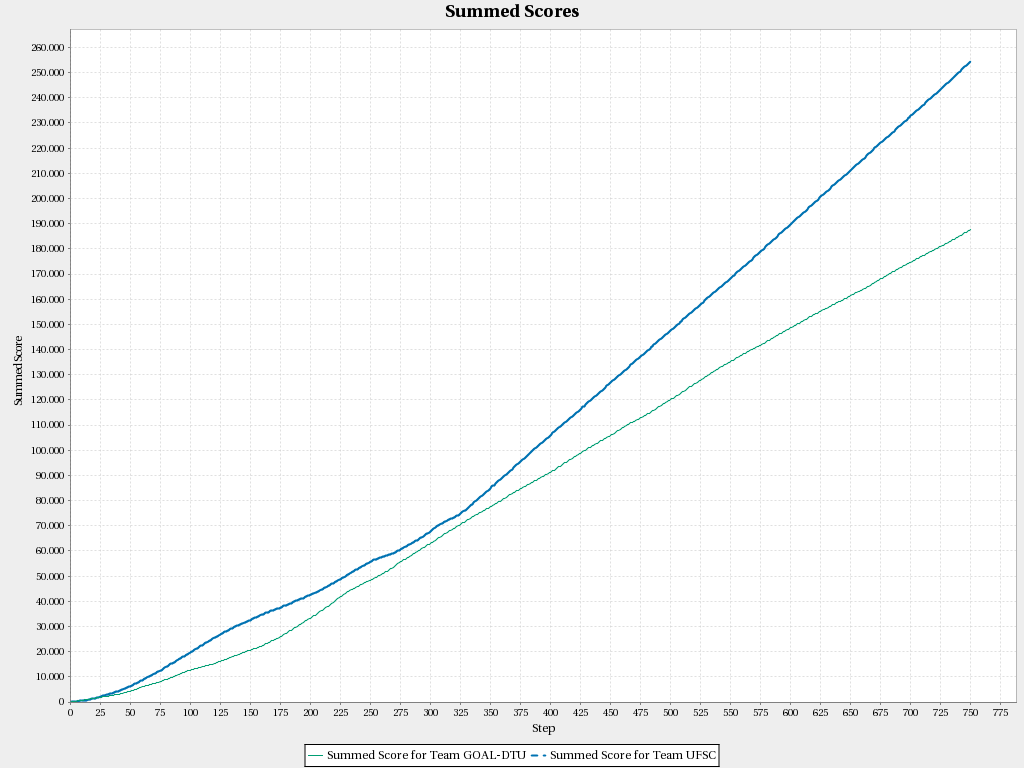
\includegraphics[width=0.49\textwidth]{figs/Scores.png}\label{fig:Scores}}
 \subfigure[ZoneStabilities]{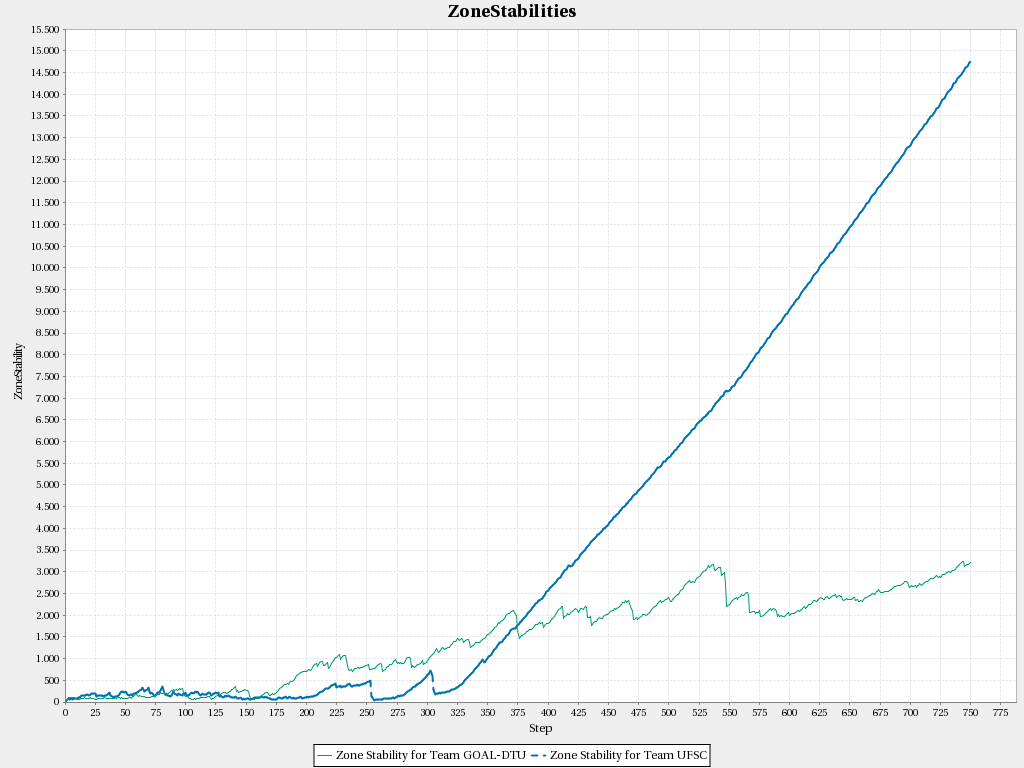
\includegraphics[width=0.49\textwidth]{figs/ZoneStabilities.png}\label{fig:ZoneStabilities}}
 \\
 \subfigure[AchievementPoints]{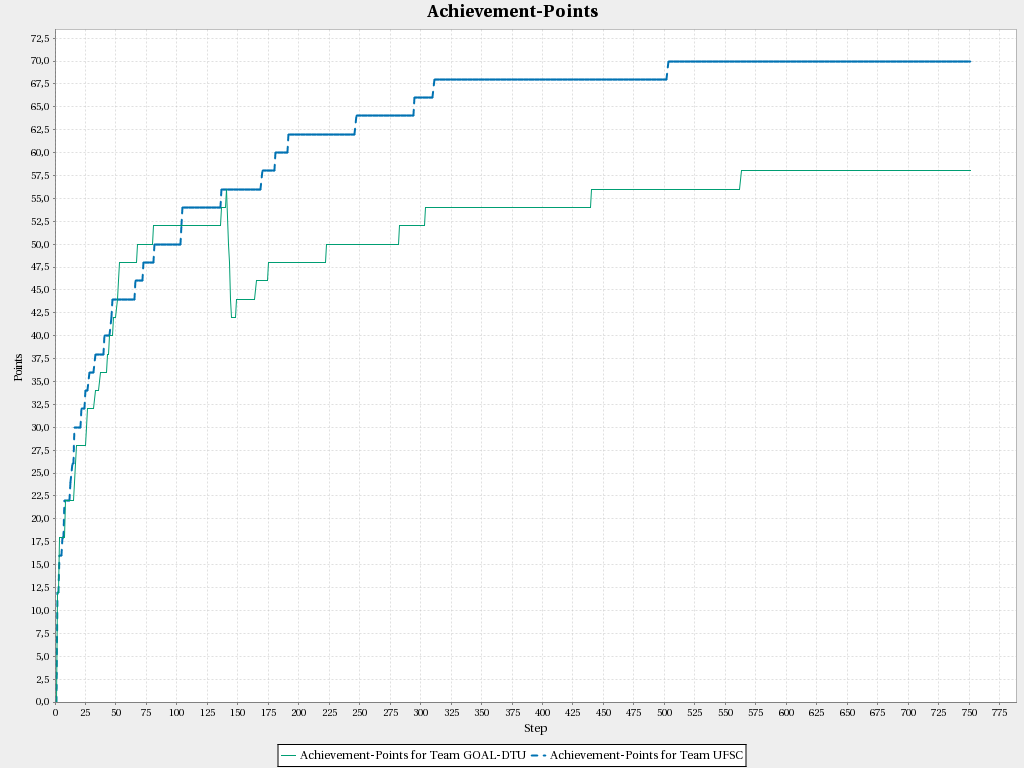
\includegraphics[width=0.49\textwidth]{figs/AchievementPoints.png}\label{fig:AchievementPoints}}
 \subfigure[ZonesScores]{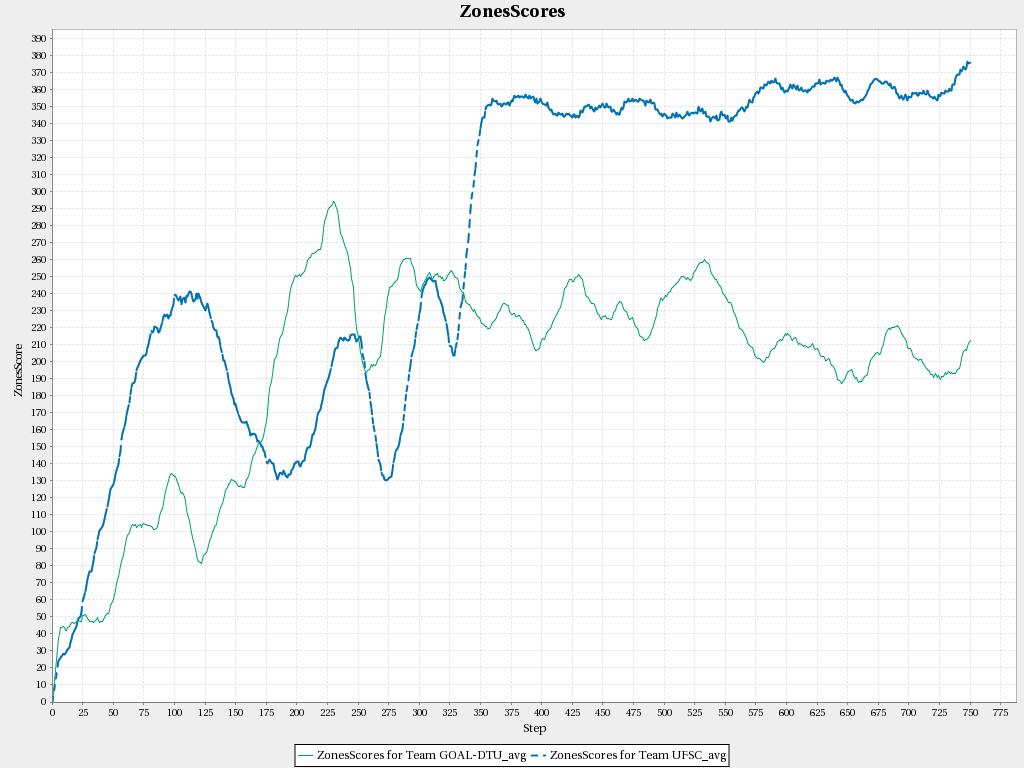
\includegraphics[width=0.49\textwidth]{figs/ZonesScores.png}\label{fig:ZonesScores}} 
 \caption{Statistics}
 \label{fig:statistics}
\end{figure}

In order to highlight the main results of our strategy we chose to use some statistics of the second match against the GOAL-DTU team \footnote{\url{http://multiagentcontest.org/downloads/func-startdown/1716/}}, which got the second place. Due our strategy of small zones, we can verify in the Fig.~\ref{fig:ZoneStabilities}  that after step 325 our team (blue) kept almost the same zones until the end of the match. This behavior is usual in all matches against the other teams. The reason is that no matter what the opponent does, our agents will rarely leave their positions.

Another interesting result can be drawn from the zones scores plot (Fig.~\ref{fig:ZonesScores}). We can see that our team (blue) kept getting almost the same zone scores after step 350 and always more than the opponent. The phase of hills can also be noticed in the beginning of the match, between step 25 until around step 130, where the team is getting high scores because of the big zones. After step 130 our team started to conquer small zones (pivots and islands) and, therefore, spreading the agents out over the whole map. It is also possible to see that, sometimes, our zone scores were lower than the enemies. This was an expected behavior when the agents were still changing their positions because the explorers were still probing new vertices. We can see it after step 250 and after around step 315, where our team decreased the gain of zone scores. After probing all vertices (around step 325), the agents started to get higher scores because they defined the fixed zones and all agents were participating.

We can see the same behavior in Fig.~\ref{fig:Scores}, where the opponent score gets closer and then the difference of scores increases again. Notice that after step 325 the difference of scores increased continuously because all vertices were probed. On the other hand, in the Fig.~\ref{fig:AchievementPoints} we can see that our team always has more achievement points than the opponent after step 125. It means we are getting more points because the opponent was buying items while our team was saving money.

\bigskip

Besides the performance of the team in the contest, we made several contributions for the tools that we used in this year. In Jason, we added features to handle goals with deadlines, new mechanisms for the \texttt{.wait} internal action, and we fixed some bugs. In \moise, we added a new feature to reset organizational goals to avoid creating new schemes at runtime and we added an organizational monitor accessed via HTTP, so that we were able to watch our team organization remotely.


The source code of the team has 3794 lines of Jason code, 135 for \moise, 96 for \cartago, and 4434 for Java, totaling 8459 lines. Although the implemented strategies of these year are more complex, we can notice that the number of lines coded in Jason has decreased from 5504 in last year's team to 3794 this year. It is an expected consequence of the organization and the environment programming available in \jacamo. Coordination strategies that previously required several lines of Jason code, could now be coded in a few lines of \moise, since \moise\ is a proper language for that.  Not only have we reduced the size of the programs, but the new approach has allowed us to debug and change the organization of the team quite easily. Instead of monitoring the agents internal state, we can now monitor the state of the organization, which is a more general view of the state of the team. Since the organizational program is the same as the specification, to change the team sometimes is simply reduced to update the organization. For instance, to change the order of organizational goals, we simply need to change the scheme of Fig.~\ref{fig:org_fs}.  
\section{Conclusion}

In our second participation in the MAPC we had again a worthy experience. Our team performed very well and we won the MAPC for the second consecutive year. The strategy to get many small zones was the strongest point of our team and it became more difficult for the opponents to disturb our zones because our agents were spread out over the whole map while our saboteurs were able to disturb the opponent zones. However, our team can be improved to perform better in maps with low thinning (less than 20\%) and with too many good vertices gathered in the same area. The best strategy for it seems to be to conquer a big zone and defend it instead of building small zones.

We also had the opportunity to use new tools, such as the \jacamo\, and to test some issues related to our research topics, such as \emph{count-as rules}. It was a good challenge and we got positive results. The main results were ($i$) the contributions for the improvement of the used tools and ($ii$) the concrete verification that considering the organization and the environment as first-class entities has improved the team program quality.

Finally, as suggestions to improve the current scenario, we suggest that ranged actions be revised to balance the fail probability. So far, it is not a good strategy to use ranged actions, since the agents need to buy several sensors to decrease this probability. 	

\bibliographystyle{plain}
\bibliography{bibliografia}

\section*{Short Answers}

\appendix

\section{Introduction}

\begin{enumerate}
\item What was the motivation to participate in the contest?\\
	A: Evaluate the result of our master and PhD thesis.

%Multi-Agent Programming Contest offers an useful context based on cooperation, coordination, and decentralisation to evaluate our master and Phd thesis proposals. Our main approach is ($i$) to develop a \emph{base} multi-agent system for the contest, after it ($ii$) change the base system using our corresponding proposals, and then ($iii$) evaluate and compare  each proposal against the base system. Another motivation is to improve our experience in developing MAS, because most of us are just starting on the domain.\\

\item  What is the (brief) history of the team? (MAS course project,  thesis evaluation, $\ldots$) \\
	A: Our team was formed by members from the Multi-Agent Systems research group (called SMADAS) at Federal University of Santa Catarina (UFSC). %\\

\item  What is the name of your team?\\
	A: Our team's name is SMADAS-UFSC.%\\

\item  How many developers and designers did you have? At what level of education are your team members? \\
	A: Our team has six developers and everyone was involved with the system design. We have one PhD, one PhD student, three masters students and one undergraduate student. %\\

\item  From which field of research do you come from? Which work is related?\\
	A: All team members work with Multi-Agent Systems and Artificial Intelligence. %\\

\end{enumerate}

\section{System Analysis and Design}

\begin{enumerate}
 	\item  Did you use a Multi-Agent programming languages? Please justify your answer.\\
	A: We used the Jason language because all members are familiar with it.%\\ % and it is used in their master and PhD thesis. 
 
 	\item  If some Multi-Agent system methodology such as Prometheus, O-MaSE, or Tropos was used, how did you use it? If you did not, please justify.\\
	A: We did not use any software engineering methodology because the problem seemed quite simple to solve and we had no experience with such methodologies.%\\ %Thus we decided that it was better to use our time developing the system than learning a methodology. 
   	   
 	\item  Is the solution based on the centralisation of coordination/information on a specific agent? Conversely if you plan a decentralised solution, which strategy do you plan to use?\\
	A: The system information is decentralised: each agent has all available information about the enemies and the graph. The coordination is centralised in a few cases, to solve some conflicting situations, like defining which agent should be repaired first or what is the best zone to exploit. %\\
   
	\item  What is the communication strategy and how complex is it?\\
	A: The agents use two mechanisms for communication: a blackboard and message exchanging. Some communication protocols are composed by one single message sent by an agents to others (e.g., when an enemy is inspected or when an agent report its action). Other protocols use more messages, for example when a damaged agent request a repair, nine messages are sent among the damaged agent and the repairers.%\\
		  
    \item  How are the following agent features considered/implemented: \emph{autonomy}, \emph{proactiveness}, \emph{reactiveness}?\\
	A: The agents are autonomous, reactive, and proactive. They have autonomy to decide how and when to execute their actions, they react to environment events and new messages, and are proactive while looking for a better vertex.%\\


	\item  Is the team a truly \textbf{multi}-agent system or rather a centralised system in disguise?\\
	A: The tasks of the team are decentralised among the agents which need to coordinate themselves to produce a coherent global behaviour.%\\
	
	
	\item  How much time (man hours) have you invested (approximately) for implementing your team?\\
	 A: We expended about 500 hours developing the system.%\\


	\item  Did you discuss the design and strategies of you agent team with other developers? To which extend did your test your agents playing with other teams.\\
	A: We did not discuss the design or strategy with other teams before the contest.%\\ % because we tested different strategies in order to decide which would be used in the contest. 
	
\end{enumerate}

\section{Software Architecture}

\begin{enumerate}
	\item  Which programming language did you use to implement the Multi-Agent system?\\
	A: The language used for programming our agents is Jason 1.3.8 \cite{bordini:2007}.%\\
	
	\item  How have you mapped the designed architecture (both Multi-Agent and individual agent architectures) to programming codes, i.e., how did you implement specific agent-oriented concepts and designed artifacts using the programming language?\\
	A: The BDI concepts provided by the Jason language are the building blocks to develop our strategies.%\\ %It allows the creation of plans so the agents can complete their goals and the implementation of more than only one strategy, each one described by a plan. Our agent communication has two ways: agent to environment and agent to agent. In the first situation in each step the framework EISMASSim receives a XML file with the percepts of the agents. The agent-to-agent communication uses the Jason's performative communication.
	
	\item  Which development platforms and tools are used? How much time did you invest in learning those?\\
	A: We used Eclipse platform with Jason 1.3.8 plug-in. These tools were known by all team members then we spend just few hours learning new features. %\\
	
	\item  Which runtime platforms and tools (e.g. Jade, AgentScape, simply Java, $\ldots$) are used? How much time did you invest in learning those?\\
	A: We used EISMASSim framework to communicate with the environment and spent about 50 hours to learn it. For communication among the agents, we used Jason centralised infrastructure.%\\
		
	\item  What features were missing in your language choice that would have facilitated your development task?\\
	A: The Jason language has almost all features we needed to program our agents. However, for some algorithms, we preferred Java because it is faster.%\\
	
	\item  Which algorithms are used/implemented?\\
	A: We used two traditional algorithms for graphs: Dijkstra and breadth-first search.%\\ %algorithm to find the best path between vertices. The second is the breadth-first search algorithm to locate the best area in the graph. These algorithms were implemented using Java methods and our BDI agents used internal actions to invoke these methods.
	
	\item  How did you distribute the agents on several machines? And if you did not please justify why.\\
	A: The agents were conceived to execute in the same machine to simplify blackboard programming, which uses shared memory. Future versions of the system will use distributed blackboards.%\\
		
	\item  To which extend is the reasoning of your agents synchronized with the receive-percepts/send-action cycle?\\
	A: The synchronisation with the environment is given by the reasoning cycle of Jason, where the first step includes the perception and the last the action.%\\
		
	\item  What part of the development was most difficult/complex? What kind of problems have you found and how are they solved?\\
	A: A blackboard has been used to share and build the knowledge about the environment. The process to update information in the graph has a high computational cost, lasting more than one step. Therefore, to avoid losing steps, the graph is updated and shared every three steps.%\\
		
	\item  How many lines of code did you write for your software?\\
	A: We have 7885 lines of code, 5504 written in Jason and 2381 written in Java.%\\
		
		
\end{enumerate}

\section{Strategies, Details and Statistics}

\begin{enumerate}
	\item  What is the main strategy of your team?\\
	A: We conceived our system strategy in two main phases: exploration, in which the explorers identify all vertices and nodes in the map and the best zones, and exploitation, where all agents try to conquest and defend these zones.%\\
	 
 	\item  How does the overall team work together? (coordination, information sharing, ...)\\
	A: Our agents exchange information to coordinate their activities.%\\ %This information exchange also helps to prevent redundant actions.

	\item  How do your agents analyse the topology of the map? And how do they exploit their findings?\\
	A: Some important information about the graph structure is shared and synchronized in the blackboard and it is used by the agents to move through the map. Despite this, agents do not use any information about topology to make the decisions. %\\

	\item  How do your agents communicate with the server? \\
	A: We use the EISMASSim framework to communicate with the server. External actions and usual perception are used by the agents to interact with the EISMASSim.%\\

	
	\item  How do you implement the roles of the agents? Which strategies do the different roles implement?\\
	A: The implemented strategies for each agent type is shown in Table~\ref{tab:tabStrategies}.%\\
	
	\item  How do you find good zones? How do you estimate the value of zones?\\
	A: The system uses a modified version of the BFS algorithm to find the best zones in the map. It is run for all vertices, summing their values until some depth. The vertex with the highest sum represents where the best zone is (zone 1). After it, the algorithm tries to find the second best vertex to set the second best zone (zone 2).%\\ %This algorithm is not optimal because its result is always a circular shape, when often the ideal choice is a free shape.


	\item  How do you conquer zones? How do you defend zones if attacked? Do you attack zones?\\
	A: With the zones defined, each agent is informed about the central vertex of its zone and how far they can travel inside it. The distance they can travel is the shortest path, in  number of edges, between the central vertex and the target vertex. To defend these zones, the saboteurs attack all opponents inside the zone or in nearby vertices. The other agents stay in a vertex that has two neighbour vertices that belongs to our system. It is assumed that if the enemy zone is not near, the opponent likely has a small zone and then our agents do not try to attack it.%\\


	\item  Can your agents change their behaviour during runtime? If so, what triggers the changes?\\
	A: If the opponent does not have any buying strategy, the \texttt{Hulk} agent changes its behaviour and it stops buying upgrades. Besides it, in the start of the match the saboteurs attack the enemies, but after some steps they change their behaviour to attack the enemies. %\\


	\item  What algorithm(s) do you use for agent path planning? \\
	A: We used Dijkstra to path planning.%\\


	\item  How do you make use of the buying-mechanism?\\
	A: It was defined the minimum that the agents have to buy in order to make the enemy expend its money. In particular, we have \emph{one} agent (named \texttt{Hulk}) that focus on buying and inducing all the opponents to also buy and spend their money.%\\ %One agent (named \texttt{Coach}) was chosen to receive information about the opponents and if necessary this agent informs to \texttt{Hulk} to stop buying. 


	\item  How important are achievements for your overall strategy?\\
	A: The achievement points are quite important since they accumulate each step. It is desirable to get the maximum of achievement points as soon as possible, but some achievements are hard to get. For example, our system does not surveys all edges and they do not inspect all opponents because it takes a long time and it is better to keep the agents in the best vertices, getting water wells score. %\\


    \item  Do your agents have an explicit mental state?\\
	A: The agents have their beliefs and use them to reason about their next action.%\\ %The agents also keep in their beliefs base many information to exchange with other agents.


	\item  How do your agents communicate? And what do they communicate?\\
	A: Our agents communicate indirectly by using the blackboard and directly by message exchanging. %\\ %In the blackboard all information about the graph structure is synchronized. By the message exchanging the agents transmit informations about the enemies, friends, executed actions, damages, map zones, vertices and edges. 
	
	\item  How do you organize your agents? Do you use e.g. hierarchies? Is your organization implicit or explicit?\\
	A: There is an explicit pre-defined hierarchy to prevent redundant actions: agents with higher priority decide before the others.%\\


	\item  Is most of your agents’ behavior emergent on an individual or team level?\\
	A: In our strategy both individual and group behaviour are important. The individual behaviour is important when the agents are isolated in the map trying to get achievement points. The group behaviour is responsible for preventing redundant actions and conquering zones, for example.%\\


	\item  If your agents perform some planning, how many steps do they plan ahead?\\
	A: We do not use planning, all plans are previously programmed based on the strategies. %\\
          %Our agents do not plan a lot of steps ahead because the environment changes fast, and so the plans must be adapted to it. In most cases the agents react in just one step. Some situations when they plan with some steps ahead is when there is a disabled agent or unprobed vertex. 

	\item  If you have a perceive-think-act cycle, how is it synchronized with the server? \\
	A: We use the EISMAssim framework \cite{behrens:2011} to synchronize the agent actions to the server.%\\
	
\end{enumerate}

\section{Conclusion}
\begin{enumerate}
	\item  What have you learned from the participation in the contest?\\
	A: We learned a lot about MAS developing and about the tools and languages we used. %\\
		
	\item  Which are the strong and weak points of the team?\\
	A: Our strongest point is that we created several strategies for each system feature and  tested them against each other to select the more efficient ones. Our weakness is that our system is not so offensive. Another problem is that our agents does not focus on defending their own zone.%\\
		
	\item  How suitable was the chosen programming language, methodology, tools, and algorithms?\\
	A: The Jason programming language was quite mature and suitable for the agent programming. However, we still need tools for programming and debugging at a higher level of abstraction.%\\ %supports agent programming with abstract concepts like plans, beliefs, and goals which are suitable for the problem and very expressive. We did not identify any bug on Jason which shows the maturity of this kind of language. Although we can evaluate the used tools positively in general, some features are still missing. For example, it was very difficult to change, refactor, and debug the agents code. The tools provided by Jason for debugging, like the sniffer and the mind inspector, are too specific and focused on the details.

	\item  What can be improved in the contest for next year?\\
	A: We can improve our system both in the strategies and the tools. Our system is focused only on the agent aspect and more global aspects should be considered.%\\ %, for instance, for organisation and interaction programming as first class abstractions.
	
	\item  Why did your team perform as it did? Why did the other teams perform better/worse than you did?\\
	A: Our system performed well because we focused on extensively testing all strategies. %\\
	
	\item  Which other research fields might be interested in the Multi-Agent Programming Contest?\\
	A: We think that some parts of the problem can be solved by optimisation techniques, which we plan to use in future versions of the systems.%\\
	
	\item  How can the current scenario be optimized? How would those optimizations pay off? \\
	A: We propose two improvements. ($i$) Inform opponent's score. It would allow participants to design strategies based on the current match result, rising more confrontations. ($ii$) Leave the graph less connected to increase the use of edges.%\\ %Currently the edges do not influence the system strategies but a less connected graph forces the systems to work with the edges weight.
	
	
\end{enumerate} 
%---------------------------------
%MAX PAGES = 10
\end{document}
